\newpage
\hypertarget{emptyPartition tex}{}
\subsection{Implementing empty}
\texHeader

\begin{itemize}
 
\item[$\blacktriangleright$] To initialize your new control flow, you can once again take advantage of eMolfon's auto completion. Inside the
\texttt{empty} declaration, press  \texttt{ctrl + space} and select \texttt{forEach} from the menu (Fig.~\ref{fig:typeCompletion}).

\vspace{1cm}

\begin{figure}[htpb]
\begin{center}
  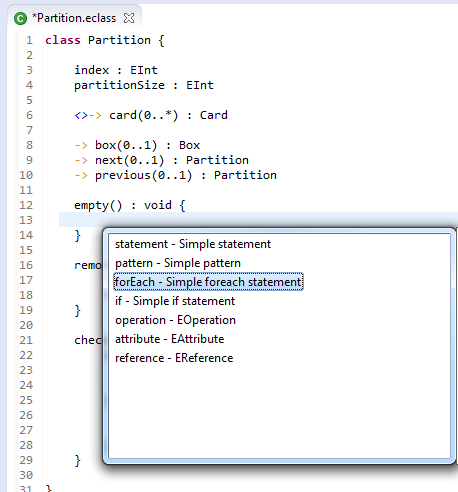
\includegraphics[width=0.7\textwidth]{eclipse_emptyTypeCompletion}
  \caption{eMoflon's auto completion}
  \label{fig:typeCompletion}
\end{center}
\end{figure}

\vspace{1cm}

\item[$\blacktriangleright$] Create a single pattern, \texttt{deleteCardsInPartition}. Remove the suggested second pattern as you only need to complete the
deletion -- no extra steps are required in this simple case!

\item[$\blacktriangleright$] Your activity should now resemble Fig.~\ref{fig:emptyControlFlow}.

\clearpage

\begin{figure}[htpb]
\begin{center}
  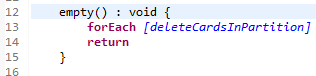
\includegraphics[width=0.5\textwidth]{eclipse_emptyControlFlow}
  \caption{Control flow for \texttt{partition.empty()}}
  \label{fig:emptyControlFlow}
\end{center}
\end{figure}

\item[$\blacktriangleright$] While similar to \texttt{removeCard}, this new pattern goes one step further by requesting a full destruction of \texttt{card},
instead of just detaching the link. This means that, in addition to destroying the link between the partition and \texttt{card}, we need a to destroy the object
variable.

\item[$\blacktriangleright$] Create a \texttt{@this} object variable, and delete its link to \texttt{card} with \texttt{-~- -> card:card}. Then create another
object variable \texttt{card}, deleting its by prefacing its name with the \texttt{-~-} operator.

\vspace{0.5cm}

\item[$\blacktriangleright$] Your pattern should now resemble Fig.~\ref{fig:emptyPattern}.

\vspace{0.5cm}

\begin{figure}[htpb]
\begin{center}
  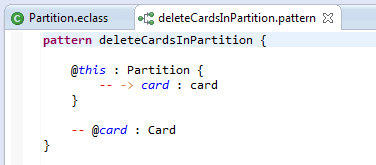
\includegraphics[width=0.6\textwidth]{eclipse_emptyPattern}
  \caption{Destroying an entire card}
  \label{fig:emptyPattern}
\end{center}
\end{figure}

\item[$\blacktriangleright$] That's it! Look at you go, you're just speeding through these SDMs now! To see how \texttt{empty} is specified in the visual
syntax, review Fig.~\ref{fig:sdm_end} from the previous section.

\item[$\blacktriangleright$] Although the Learning Box GUI does not have an explicit action that invokes this SDM, feel free to extend it and see your SDM in
action.

\end{itemize}
